\documentclass{report}
\usepackage{hyperref}
\usepackage{listings}
\usepackage{graphicx}
\usepackage[affil-it]{authblk}
\usepackage{color}
\usepackage{float}
\usepackage{wrapfig}

\usepackage{tikz}
\usepackage[bottom]{footmisc}

\usepackage{pifont}
\usepackage{tcolorbox}
\usepackage{tabularx}
\usepackage{array}
\usepackage{colortbl}
\tcbuselibrary{skins}

\author{Dominik Peuscher}
\title{Solution To The Expression Problem With SugarJ}
\date{2014}
\affil{Department of Computer Science\\ University of Marburg}

\newcommand{\Hiline}{\makebox[0pt][l]{\color[rgb]{1,0.96,0.98}\rule[-4pt]{\linewidth}{12.5pt}}}

\newcommand{\Hilinered}{\makebox[0pt][l]{\color[rgb]{1,0.96,0.96}\rule[-4pt]{\linewidth}{12.5pt}}}
\newcommand{\Hilineyellow}{\makebox[0pt][l]{\color[rgb]{1,1,0.96}\rule[-4pt]{\linewidth}{12.5pt}}}
\newcommand{\Hilinegreen}{\makebox[0pt][l]{\color[rgb]{0.96,1,0.96}\rule[-4pt]{\linewidth}{12.5pt}}}
\newcommand{\Hilinecyan}{\makebox[0pt][l]{\color[rgb]{0.96,1,1}\rule[-4pt]{\linewidth}{12.5pt}}}
\newcommand{\Hilineblue}{\makebox[0pt][l]{\color[rgb]{0.96,0.96,1}\rule[-4pt]{\linewidth}{12.5pt}}}
\newcommand{\Hilinepurple}{\makebox[0pt][l]{\color[rgb]{1,0.96,0.9}\rule[-4pt]{\linewidth}{12.5pt}}}

\newcommand{\Hilineredsmall}{\makebox[0pt][l]{\color[rgb]{1,0.96,0.96}\rule[-4pt]{0.93\linewidth}{12.5pt}}}
\newcommand{\Hilineyellowsmall}{\makebox[0pt][l]{\color[rgb]{1,1,0.96}\rule[-4pt]{0.93\linewidth}{12.5pt}}}
\newcommand{\Hilinegreensmall}{\makebox[0pt][l]{\color[rgb]{0.96,1,0.96}\rule[-4pt]{0.93\linewidth}{12.5pt}}}
\newcommand{\Hilinecyansmall}{\makebox[0pt][l]{\color[rgb]{0.96,1,1}\rule[-4pt]{0.93\linewidth}{12.5pt}}}
\newcommand{\Hilinebluesmall}{\makebox[0pt][l]{\color[rgb]{0.96,0.96,1}\rule[-4pt]{0.93\linewidth}{12.5pt}}}
\newcommand{\Hilinepurplesmall}{\makebox[0pt][l]{\color[rgb]{1,0.96,0.98}\rule[-4pt]{0.93\linewidth}{12.5pt}}}

\newcommand{\Hilineredsmaller}{\makebox[0pt][l]{\color[rgb]{1,0.96,0.96}\rule[-4pt]{0.86\linewidth}{12.5pt}}}
\newcommand{\Hilineyellowsmaller}{\makebox[0pt][l]{\color[rgb]{1,1,0.96}\rule[-4pt]{0.86\linewidth}{12.5pt}}}
\newcommand{\Hilinegreensmaller}{\makebox[0pt][l]{\color[rgb]{0.96,1,0.96}\rule[-4pt]{0.86\linewidth}{12.5pt}}}
\newcommand{\Hilinecyansmaller}{\makebox[0pt][l]{\color[rgb]{0.96,1,1}\rule[-4pt]{0.86\linewidth}{12.5pt}}}
\newcommand{\Hilinebluesmaller}{\makebox[0pt][l]{\color[rgb]{0.96,0.96,1}\rule[-4pt]{0.86\linewidth}{12.5pt}}}
\newcommand{\Hilinepurplesmaller}{\makebox[0pt][l]{\color[rgb]{1,0.96,0.98}\rule[-4pt]{0.86\linewidth}{12.5pt}}}

\newcommand{\Hilineredsmallest}{\makebox[0pt][l]{\color[rgb]{1,0.96,0.96}\rule[-4pt]{0.79\linewidth}{12.5pt}}}
\newcommand{\Hilineyellowsmallest}{\makebox[0pt][l]{\color[rgb]{1,1,0.96}\rule[-4pt]{0.79\linewidth}{12.5pt}}}
\newcommand{\Hilinegreensmallest}{\makebox[0pt][l]{\color[rgb]{0.96,1,0.96}\rule[-4pt]{0.79\linewidth}{12.5pt}}}
\newcommand{\Hilinecyansmallest}{\makebox[0pt][l]{\color[rgb]{0.96,1,1}\rule[-4pt]{0.79\linewidth}{12.5pt}}}
\newcommand{\Hilinebluesmallest}{\makebox[0pt][l]{\color[rgb]{0.96,0.96,1}\rule[-4pt]{0.79\linewidth}{12.5pt}}}
\newcommand{\Hilinepurplesmallest}{\makebox[0pt][l]{\color[rgb]{1,0.96,0.98}\rule[-4pt]{0.79\linewidth}{12.5pt}}}

\newcommand{\HilineBackground}{}
\newcommand{\HilineTypessmall}{}
\newcommand{\HilineTypessmaller}{}
\newcommand{\HilineMethodssmall}{}
\newcommand{\HilineMethodssmallest}{}
\newcommand{\HilineAlgebrasmall}{}


\begin{document}
\lstdefinelanguage{exprExt}{alsolanguage=java, morekeywords={family}}
\lstset{
 frame=single,
 frameround=tttt,
 framexleftmargin=8mm,
 keywordstyle=\bfseries\ttfamily\color[rgb]{0.6,0,0.6},
 identifierstyle=\ttfamily,
 commentstyle=\color[rgb]{0.5,0.5,0.5},
 stringstyle=\ttfamily\color[rgb]{0,0,1},
 showstringspaces=false,
 basicstyle=\normalsize,
 numberstyle=\footnotesize,
 numbers=left,
 stepnumber=1,
 numbersep=10pt,
 tabsize=2,
 breaklines=true,
 prebreak = \raisebox{0ex}[0ex][0ex]{\ensuremath{\hookleftarrow}},
 breakatwhitespace=false,
 aboveskip={1.5\baselineskip},
 columns=fixed,
 upquote=true,
 extendedchars=true,
 escapechar=^}

\maketitle

\tableofcontents
\listoffigures

\chapter*{Abstract}


\chapter*{Preface}

This paper is written as part of a bachelors degree. The engineered result, examples and use cases are published on Github.com\cite{Peuscher-GitHub-EP-2014}.% We take the equality of people of different genders very serious. We chose to refer in general to a male reader in terms of readability. Every mention of a male reader is meant to be gender-neutral.



%%%%%%%% Introduction
\chapter{Introduction}

We extend Java with a specific syntax for the \emph{Expression Problem} (EP). Therefore we use a solution of the EP which has been modified so that much of the boilerplate code can be generated. The resulting solution is difficult for users to understand and adapt to their needs. We overcome this difficulty, by defining a new syntax that is easier to understand. It is then transformed into valid Java code. The new syntax and the transformation to Java is implemented in a \emph{SugarJ library}. This approach is meant to simplify the use of a solution to the EP.

The Expression Problem is a name that was proposed by Philip Wadler \cite{Wadler-Expression-1998}. It refers to the problem of adding both new types and new operations to a given code-structure. Generally, \emph{object-oriented languages} make it easy to add new types to code and \emph{function languages} make it easy to add new operations to code (this extendibility is a key feature of modern programing languages). Classes inherit from other classes in object-oriented languages and functions inherit from other functions in functional languages. These are the two dimensions of Inheritance. The Expression Problem is found in both functional and object-oriented languages and it occurs when one tries to extend a data structure in both dimensions. This thesis uses a solution that overcomes this problem in the object-oriented language Java.

There are many papers that present solutions to this problem. The solution developed in this thesis is a modification of the solution proposed by Oliveira et. al., which enables much of the boilerplate code to be  easily generated \cite{Oliv-Extensibility-2012}. The modifications made to Oliveira et. al.'s solution includes the use of stateful objects and the use of \emph{delegation} instead of combined object algebras to allow dependent methods.

Extending a programming language (which is Java in this case) with new syntax is a way to support special use cases with a fixed pattern. The syntax and their extension is specified in \emph{syntax definition formalism} (SDF), which uses the definitions of a \emph{context free language} (CFL) \cite{Heering-SDF-1989}. The code in the extended syntax is parsed using these rules and generates an \emph{ATerm} \cite{Brand-ATerms-2000}. This \emph{ATerm} is the representation of the program in the extended language. To get valid Java from this extended language \emph{Stratego} rules are used to rewrite the \emph{ATerm}. The \emph{Stratego} rules are the formal representation of the solution to the EP. After the application of the solution the \emph{ATerm} can be pretty-printed into valid Java code. The process from parsing the new syntax to printing it out to Java is managed by \emph{SugarJ} \cite{Erdweg-SugarJ-2011}.

\emph{SugarJ} is a language extension framework that uses \emph{SDF}, \emph{Stratego} and the \emph{Spoofax framework} \cite{Kats-Spoofax-2010}. It can be used with \emph{integrated development environments} (IDE) to support syntax highlighting for the new syntax. The generated code does not depend on \emph{SugarJ} and so allows collaborative work across different environments. This thesis is also a case study, which outlines the experiences gained using SugarJ (a relatively young framework) to develop the syntax extension. I will also give the reader an impression of the time and effort required to use SugarJ.










%%%%%%%%% Solution to the Expression Problem
\chapter{Solution to the Expression Problem}

\section{Methods}

%%%%%% The Problem
\subsection{The Problem}
\label{theProblem}

Although the problem was discussed as early as 1975 by Reynolds, the name "\emph{Expression Problem}" was proposed by Wadler in 1998 on the Java Genericity Mailing List \cite{Reynolds-Abstraction-1975, Wadler-Expression-1998}. The Expression Problem is a problem of extensibility. An extension of code means either adding new types that implement a fixed interface or alter an interface to support new operations. In \emph{object-oriented programming} (OOP) it is easy to add new types. A type is declared to implement an interface and the existing interface and classes do not have to be modified or recompiled. To add new operations one would have to alter the existing interfaces and classes, which might be erroneous or not even possible (e.g. when the source code is not available). By extending both (interfaces and classes) the static type safety is not ensured. Using \emph{casts} could fix this, however, it will lead to an increased risk of runtime exceptions.

The requirements on a solution to the problem are proposed by Wadler and Zenger et. al. \cite{Wadler-Expression-1998, Odersky-Expression-2005, Oliv-Extensibility-2012}. Only when a solution meets all of the requirements can it be considered a valid solution. The requirements are:

\begin{itemize}
  \item \emph{Extensibility in both dimensions}: A solution must allow the addition of new data variants and new operations and support extending existing operations.
  \item \emph{Strong static type safety}: A solution must prevent applying an operation to a data variant, which it cannot handle using static checks.
  \item \emph{No modification or duplication}: Existing code must neither be modified nor duplicated.
  \item \emph{Separate compilation}: Safety checks or compilation steps must not be deferred until link or runtime.
  \item \emph{Independent extensibility}: It should be possible to combine independently developed extensions so that they can be used jointly.
\end{itemize}


%%%%%% Running Example
\subsection{Running Example}

To clarify the problem and the solution we use an example that is used in much of the literature about the EP. The example consists of simple abstract mathematical expressions (e.g. 1 + 2) with two types: \emph{Literals} (in this case natural numbers: 1, 2, 3, ...) and the \emph{Add operation}. The base package\footnote{It is not mandatory a \emph{package}. We consider \emph{package} as editable entity} only consists of the lit-object with a print-method (Figure \ref{exampleLitBaseClass}).


\begin{figure}[H]
\begin{lstlisting}[language=java]
interface Methods {
    public String print();
}
class Lit implements Methods {
    private Integer x;
    public Lit(Integer x) { this.x = x; }
    public String print() { return x.toString(); }
}
\end{lstlisting}
\caption{Static \textbf{base package}: a simple \lstinline{Lit}-class with \lstinline{print} operation that is to be extended}
\label{exampleLitBaseClass}
\end{figure}
\begin{figure}[H]
\begin{lstlisting}[language=java]
interface Methods2 extends Methods {
    public Integer count();
}
class Lit2 extends Lit implements Methods2 {
    public Integer count() { return 1; }
}
\end{lstlisting}
\caption{\textbf{First extension}: Adding the new operation \lstinline{count} to \lstinline{Lit} from the base package}
\label{exampleFirstExtension}
\end{figure}

The \emph{first extension} extends the base package by a new \emph{operation}. With the new operation \lstinline{count}\footnote{\lstinline{count} counts the amount of connected symbols in the expression} we need to extend the interface with the operation and create a new type \lstinline{Lit2} that implements the new interface (see figure \ref{exampleFirstExtension}).

The \emph{second extension} extends the base package by a new \emph{type}. We create the new type \lstinline{Add} and implement the interface of the base package \lstinline{Methods} (See figure \ref{exampleSecondExtension}).

The \emph{third extension} combines the \emph{first extension} and the \emph{second extension}. We create the new type \lstinline{Add2} that needs to cast calls to the \lstinline{left}- and \lstinline{right}-fields to \lstinline{Methods2} to exectute the \lstinline{count} operation on them (See figure \ref{exampleThirdExtension}. This violates the requirement for \emph{Strong static type safety} (see section \ref{theProblem}).

\begin{figure}[H]
\begin{lstlisting}[language=java]
class Add implements Methods {
    protected Methods left;
    protected Methods right;
    public Add(Methods left, Methods right) {
        this.left = left;
        this.right = right;
    }
    public String print() {
        return left.print() + "+" + right.print();
    }
}
\end{lstlisting}
\caption{\textbf{Second extension}: Adding the new type \lstinline{Add} that implements \lstinline{Methods} from the base package}
\label{exampleSecondExtension}
\end{figure}
\begin{figure}[H]
\begin{lstlisting}[language=java,commentstyle=\color{red}]
class Add2 extends Add implements Methods2 {
    public Add2(Methods2 left, Methods2 right) {
        super(left,right);
    }
    public Integer count() {
        return 1 + (/*CAST*/(Methods2)left).count() 
                 + (/*CAST*/(Methods2)right).count();
    }
}
\end{lstlisting}
\caption{\textbf{Third extension}: Combining the \emph{first} and \emph{second} extension is only possible with \lstinline{Methods2}-cast, because \lstinline{left} and \lstinline{right} are of \lstinline{Methods} which do not know an operation \lstinline{count}}
\label{exampleThirdExtension}
\end{figure}

\begin{figure}[H]

\includegraphics[width=330px,keepaspectratio=true]{Expression_problem-diag.jpg}

\caption{UML class diagram of the example}
\label{exampleClassDiagram}
\end{figure}

%%%%%% Solution: Extensibility for the Masses

\subsection{Solution: Extensibility for the Masses}

The solution by Oliveira et. al. \cite{Oliv-Extensibility-2012} is an approach that uses \emph{Object Algebras}. Object algebras are related to the \emph{Abstract Factory} pattern, that is a way to inject dependencies \cite{Gof-Design-1993}. The dependency injection with object algebras solves the requirement for \emph{Strong static type safety} (see section \ref{theProblem}). The other requirements are met by decoupling the operations from their generic Java types and creating an extra result type for every result of an operation (see figure \ref{differentAlgebras}). This elegantly bypasses most of the requirements including the requirement of \emph{Independent extensibility}, which is difficult to comply with.

\begin{figure}[h]
\begin{lstlisting}[language=java]
    <A> A exp(IntAlg<A> v) {
        return v.add(v.lit(3), v.lit(4));
    }
    void test() {
        IntFactory base = new IntFactory();
        IntPrint print = new IntPrint();
        int x = exp(base).eval();// int x = exp.eval();
        String s = exp(print).print();
    }
\end{lstlisting}
\caption{Extensibility for the Masses \cite{Oliv-Extensibility-2012} pages 8, 9. Every Operation has its own result type. The \emph{object algebra} decides the result type. \lstinline{IntFactory} returns an object with \lstinline{eval}-operation, \lstinline{IntPrint} returns an object with \lstinline{print}-operation}
\label{differentAlgebras}
\end{figure}

The extension of types is done by extending the \emph{object algebra interface} (\lstinline{IntAlg<A>} in figure \ref{differentAlgebras}) and the \emph{object algebras} whereas the extension of operations is done with an extra object algebra for every operation.

To add new types one would extend the object algebra interface, to add new operations one would create a new create a new object algebra with a corresponding result (anonymous) class. To independently extend multiple extensions Oliveira et. al. proposed to use a special object algebra like \lstinline{Union<A>} and \lstinline{Combine<A,B>}. \lstinline{Union<A>} delegates the instantiation of result objects to the two or more different algebras that are to be combined. \lstinline{Combine<A,B>} returns a \lstinline{Pair<A,B>}-object with which operations that depend on other operations can be defined (see figure \ref{combineExampleOliv}).

This approach is very neat. However we chose not to use this solution for the following reasons:

\begin{itemize}
  \item \emph{Surrounding code}: Developers that write the surrounding code need a great deal of knowledge about the solution and its inner implementation. They do not get an interface that concludes all operations and they have to decide which interface brings which operation (see figure \ref{combineExampleSurrounding}).
  \item \emph{Complexity}: The proposed extension relies on nesting the \lstinline{Union<A>}- and \lstinline{Combine<A,B>}-algebras and the \lstinline{Pair<A,B>}-result. This would become very complex. Our aim is to have a solution that can easily be generated and that does not seem possible with the complexity of this solution.
  \item \emph{Depending methods}: Oliveira et. al. presents a \lstinline{Debug} object algebra as an example of depending methods. This algebra prints out debug data on the console. There is no solution that has been shown to work with dependent methods that include a return value. We assume such a case would look like that described in figure \ref{depentendPrintTerm} which uses \emph{delegation}. However this is a very complex solution \cite{Tempero-Multiple-2000}.
\end{itemize}

\begin{figure}[H]
\begin{lstlisting}[language=java]
class Pair<A, B> {
  A a; B b;
  Pair(A a, B b) { this.a = a; this.b = b; }

  A a() { return a; }
  B b() { return b; }
}
class Combine<A, B> implements IntAlg<Pair<A, B>> {
  IntAlg<A> v1;
  IntAlg<B> v2;

  Combine(IntAlg<A> v1, IntAlg<B> v2) {
    this.v1 = v1;this.v2 = v2;
  }
  
  public Pair<A, B> lit(int x) {
    return new Pair<A, B>(v1.lit(x), v2.lit(x));
  }
  public Pair<A, B> add(Pair<A, B> e1, Pair<A, B> e2) {
    return new Pair<A, B>(
      v1.add(e1.a(), e2.a()),
      v2.add(e1.b(), e2.b()));
  }
}
\end{lstlisting}
\caption{\lstinline{Combine} use case \cite{Oliv-Extensibility-2012} page 17}
\label{combineExampleOliv}
\end{figure}

\begin{figure}[H]
\begin{lstlisting}[language=java]
Combine<Exp, IPrint> x = new Combine<Exp, IPrint>();
Pair <Exp,IPrint> p = x.add(x.lit(1),x.lit(2));
System.out.println(p.b().print() + "=" + p.a().eval());
\end{lstlisting}
\caption{The surrounding code would have to know which operation is in which part of \lstinline{Pair}}
\label{combineExampleSurrounding}
\end{figure}

\begin{figure}[H]
\begin{lstlisting}[language=java]
interface IDepends <A, B> {
  public void setPair(Pair<A, B>);
  public Pair<A, B> super();
}
class DependentCombine
    <A implements Depends<Exp, IPrint>>
    extends Combine<Exp, IPrint>
     {
  DependentCombine() {
    super(new IntFactory(), new IntPrint());
  }
  public A lit(int x) {
    A dependent = new A();
    dependent.setPair(new Pair(v1.lit(x),v2.lit(x)));
    return dependent;
  }
  public A add(TermPair e1, TermPair e2) {
    A dependent = new A();
    dependent.setPair(return new Pair(
      v1.add(e1.a(), e2.a()),
      v2.add(e1.b(), e2.b())));
    return dependent;
  }
}

interface IPrintTerm { public String printTerm(); }
class Term implements Depends <Exp, IPrint> {
  Pair <A, B> pair;
  public setPair(Pair<Exp, IPrint> pair) {
      this.pair = pair;
  }
  public IPrintTerm printTerm() {
    final Pair <A, B> pair = this.pair;
    return new IPrintTerm() {
      public String printTerm() {
        return pair.b().print() + "="
            + pair.a().eval().toString();
      }
    };
  }
}

\end{lstlisting}
\caption{Dependent \lstinline{PrintTerm} object algebra implementation}
\label{depentendPrintTerm}
\end{figure}


%%%%%% Delegation

\subsection{Delegation for Independent Extension}

Independent extension requires some kind of \emph{multiple inheritance}. We chose not to use the solution of Oliveira et. al. because of its complexity. Instead we simulate \emph{multiple inheritance} with \emph{interface-delegation} as proposed by Tempero et. al. \cite{Tempero-Multiple-2000}.

Java does not support \emph{multiple inheritance} for classes. To support \emph{independent extensibility} without multiple inheritance, we simulate it. For every \emph{super-type} (named \emph{parent}) that is inherited from we instantiate an object\footnote{We consider every extension to be non-abstract} in the constructor. Every operation that is not implemented in the \emph{derived type} (named \emph{child}) will be explicitly delegated to the \emph{parent} and the returned result of the \emph{parent} will afterwards be returned by the \emph{child}s operation. This means that for every operation that a class has it has either its own implementation or a parent that it can delegate the operation to (see figure \ref{delegationExample}).

The combined class (\emph{child}) decides which operation is delegated to which parent. If only one of the parents implements the operation the child will delegate the call to this parent. If more than one parent implements the operation, the child has to decide to which parent it delegates the calls. In languages that support \emph{multiple inheritance} an algorithm implicitly decides from which parent an operation is inherited\footnote{The algorithm is also important on which parent \lstinline{super()}-calls are executed, if the language supports them}. A popular algorithm used for \emph{multiple inheritance} is \emph{mixin linearization} \cite{Bracha-Mixin-1990}. Applying this algorithm flattens and unifies the inheritance tree, which results in a list, that is used to determine the order of inheritance and \lstinline{super()}-calls.


\begin{wraptable}{r}{5cm}
\def\arraystretch{1.2}
\setlength\fboxsep{0.6pt}
\centering
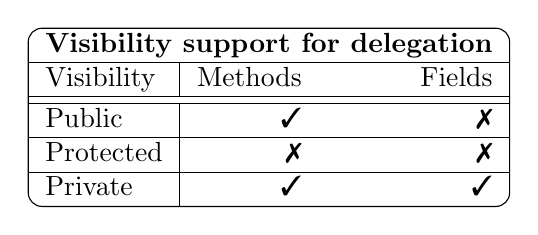
\begin{tikzpicture}
\node (table) [inner sep=0pt] {
\begin{tabular}{l|rr}
  \multicolumn{3}{c}{\cellcolor{white}\bfseries Visibility support for delegation} \\
  \hline
Visibility &  Methods & Fields   \\\hline\hline
Public     &  \ding{51} &  \ding{55} \\\hline
Protected  &  \ding{55} &  \ding{55} \\\hline
Private    &  \ding{51} &  \ding{51}
\end{tabular}
};
\draw [rounded corners=.5em] (table.north west) rectangle (table.south east);
\end{tikzpicture}
\caption{Visibility support for delegation}
\label{visibilityTable}
\end{wraptable}
Interface-delegation does not support all of Javas visibility features. Field-access cannot be delegated. Therefore public field access is only possible on the child and not on any of the parents. The biggest problem is protected access, because it is inherited with class extension. Private visibility is not meant to be inherited at all so this is not a problem for delegation. See table \ref{visibilityTable} for a quick overview.



\begin{figure}[H]
\begin{lstlisting}[language=java]
class Lit {
  private Integer _x;
  public Integer getX() {
    return _x;
  }
  public Lit(Integer X) {
    _x = x;
  }
}
class LitPrint {
  private Lit _parent;
  public LitPrint(Integer x) {
    _parent = new Lit(x);
  }
  public String print() {
    return _parent.getX().toString();
  }
}
class LitCount {
  private Lit _parent;
  public LitCount(Integer x) {
    _parent = new Lit(x);
  }
  public Integer count() {
    return 1;
  }
}
class LitPrintCount {
  private LitPrint _parentPrint;
  private LitCount _parentCount;
  public LitCount(Integer x) {
    _parentPrint = new LitPrint(x);
    _parentCount = new LitCount(x);
  }
  public Integer count() {
    return _parentCount.count();
  }
  public Integer print() {
    return _parentPrint.print();
  }
}
\end{lstlisting}
\caption{Delegation implementation of the example with the type \lstinline{Lit}}
\label{delegationExample}
\end{figure}


\section{Results}

\label{suggestedEPSolution}

\subsection{Overview}

Our Solution features a class that contains the \emph{object algebra interface}, the result class interface (\emph{aggregation interface}) and an implementation of the \emph{object algebra}. Surrounding code uses the \emph{object algebra interface} to factorize members of this family, that implement the \emph{aggregation interface}. The implementation of the factorization is the \emph{object algebra}, which can be exchanged.

\subsection{Aggregation Interface}

We use \emph{object algebras} as a factory for classes with a collection of operations (\emph{aggregation classes}). Object algebras at Oliveira et. al. return a different result interface for every operation, instead our solution returns an aggregated interface with all operations (\emph{aggregation interface}) that are needed. This makes it possible for methods of the implementing classes to depend on each other and share state variables (see figure \ref{aggregationInterfaces}).

The \emph{aggregation interface} defines all the operations the \emph{aggregation class} has, just like in general Java context. The surrounding code addresses just the \emph{aggregation interface}, there is no modification needed.

\begin{figure}[h]
\begin{lstlisting}[language=java]
    public interface Methods {
      public String print();
    }
    public interface Methods2 extends Methods {
      public Integer count();
    }
\end{lstlisting}
\caption{Aggregation interface (\lstinline{Methods}) and an extended aggregation interface (\lstinline{Methods2})}
\label{aggregationInterfaces}
\end{figure}

\subsection{Object Algebra Interface}

To generate objects based on the aggregation interface we need an object algebra, that factorizes these. This algebra needs a factory method for every type. Types are identified by their algebraic signature \cite{Oliv-Extensibility-2012}. This means, that every type is unique by its name and types of parameters. Parameters can either be abstract or concrete. Abstract parameters differ from concrete parameters so that they refer to the most specific interface in an extension hierarchy, which means the interface of the implementing object algebra. This is similar to the \emph{ThisType} extension proposed by Foster in \emph{Rupiah} \cite{Foster-Rupiah-2001}. The abstract parameter is referenced by a dynamic type parameter "A"\footnote{"A" is a convention. This only means it is dynamic mapped by the object algebra that implements the interface}. The return class of the factory methods also have the abstract type "A" as it represents the \emph{aggregation interface} (see figure \ref{algebraInterfaces}).

\begin{figure}[h]
\begin{lstlisting}[language=java]
    public interface Types <A> {
      public A lit(Integer x);
    }
    public interface Types2 <A> extends Types <A> {
      public A add(A e1,A e2);
    }
\end{lstlisting}
\caption{Interfaces for algebras with the signature of the types}
\label{algebraInterfaces}
\end{figure}

\subsection{Object Algebra}

The main part of the object algebra is to instantiate the dependencies like super-classes of a called type and then instantiate the called type and make the dependencies available. The concrete implementations of the \emph{aggregation interface} are done using anonymous classes\footnote{Anonymous classes are desugared by the Java preprocessor into real classes with all available \emph{final} variables as private fields so they can be accessed within the anonymous class} within the object algebra methods (see figure \ref{algebraImplementation}). We use this technique to keep users from specifying concrete classes instead of interface in their code, because referencing super-types does not work with \emph{delegation} which we use for \emph{multiple inheritance}.

In figure \ref{algebraImplementation} in the Lit.print()-implementation we can either use \_instance2 or \_instance3 to delegate to. Coincidentally both refer to the same operation in our example but this can differ in another environment. To find the best ancestor for delegation one should use a linearization like suggested from Bracha \cite{Bracha-Mixin-1990} for Mixins.

\begin{figure}[H]
\begin{lstlisting}[language=java]
public class Algebra4 implements Types <Methods2> {
  public Methods2 add(final Methods e1,
                      final Methods e2){
    final Methods _instance =new Algebra3().add(e1,e2);
    return new Methods2() {
             public Integer count() {
                 return e1.count() + 1 + e2.count();
             }
             public String print() {
                 return _instance.print();
             }
         };
  }
  public Methods lit(Integer x) { 
    final Methods2 _instance2 = new Algebra2().lit(x);
    final Methods _instance3 = new Algebra3().lit(x);
    return new Methods2() {
             public Integer count() { 
                 return _instance2.count();
             }
             public String print() { 
                 return _instance3.print();
             }
         };
  }
}
\end{lstlisting}
\caption{The resulting Algebra-class for the third extension (Algebra2 and Algebra3 likewise)}
\label{algebraImplementation}
\end{figure}

\subsection{Dynamic Dispatch}

As Tempero et. al. point out, there are some limits to multiple inheritance with delegation \cite{Tempero-Multiple-2000}. We worked out a workaround\footnote{The workaround is available online \cite{Peuscher-GitHub-EP-2014}} for the limit of \emph{dynamic dispatch} for \emph{dependent methods} (called \emph{self-calls} at Tempero et. al.). It has some downsides (see section \ref{discussionDynamicDispatch}) but works as expected.

The main idea of dynamic dispatch with delegation is to have a field of the original object in every delegation super-object. Therefore the original-object has to be injected into all classes.

To achieve this we have to alter the aggregation interface. We add a setter with a generic type that extends from the according \lstinline{Methods} because we do not know the last extension at this point (see figure \ref{dynamicDispatchMethods}). The visible methods of this generic type are the same as the ones from the \lstinline{Methods} interface itself.

\begin{figure}[H]
\begin{lstlisting}[language=java]
public interface Methods {
  public String print();
^\Hiline^  public <B extends Methods> void setSelfRef(B selfRef);
}
public interface Methods2 extends Methods {
  public Integer count();
^\Hiline^  public <B extends Methods2> void setSelfRef(B selfRef);
}
\end{lstlisting}
\caption{Dynamic dispatch: Adding a setter for the original object with a dynamic type \emph{B}. Needs to be done for every \lstinline{Methods} interface}
\label{dynamicDispatchMethods}
\end{figure}

With every new Methods interface a new setter has to be introduced and therefore implemented. When called, Java decides to call the method with the best matching\footnote{\emph{best matching} means if an interfaces extends another interface and both could match on a method, the method with the extending class referenced is called} interface. Therefore the setter of every super interface has to be implemented although it will not be called. The correct setter injects the original object in every super object, which do the same with their predecessors etc. Within the factory method every instance publishes itself into the super objects so sub-objects overwrites their super objects and the original object overwrites all super objects.

Dependent methods that call other methods of the calls just have to do their calls on the selfRef-object.

\subsection{Usage}
\label{combiningTheParts}
Just enumerate the interfaces and algebras would be very confusing. Therefore we suggest a form to define the interfaces and classes in a combined class (see figure \ref{combinedClass}).

To address the interface of expressions of this family, one uses \lstinline{[Familyname].Methods}. The object algebra is available with singleton pattern. This is used because the family class is not stateful and for convenience and memory usage reasons. A user calls the singleton and gets the algebra of type \lstinline{[Familyname].Types<[Familyname].Methods>} that he uses for initialization of the expression.

\subsubsection*{Extending Families}

To extend this family the developer creates a new outer class and in there the \lstinline{Methods}- and \lstinline{Types<A>}-interface\footnote{In terms of consistency the interfaces should be extended even when empty} as well as the algebra and the singleton to return the algebra instance. The \lstinline{Methods}- and \lstinline{Types<A>}-interface implement all the \lstinline{Methods}- and \lstinline{Types<A>}-interfaces of the families that should be combined. The algebra implements the \lstinline{Types<Methods>}-interface and. New types are added in the \lstinline{Types<A>}-interface (and accordingly their implementation in the algebra). The \lstinline{Methods}-interface has the setSelfRef-method (see figure \ref{dynamicDispatchMethods}) and the newly added methods. The algebra has to implement every type and in every type every method of the \lstinline{Methods}- and \lstinline{Types<A>}-interface and either implement its own methods or delegate every method call (see figure \ref{dynamicDispatchAlgebra}). All types have to be implemented, their creation is not delegated. The references have to be modified from the previous examples to meet this structure (e.g. instead of Methods2: [Familyname].Methods, instead of new Algebra2(): [Familyname].algebra(), etc.).

\begin{figure}[H]
\begin{lstlisting}[language=java]
^\HilineBackground^public class [Familyname] {
^\HilineBackground^  ^\HilineTypessmall^public interface Types<A> {
^\HilineBackground^  ^\HilineTypessmall^  [...Types...] // see figure ^\color{gray}\ref{algebraInterfaces}^
^\HilineBackground^  ^\HilineTypessmall^} 
^\HilineBackground^  ^\HilineMethodssmall^public interface Methods {
^\HilineBackground^  ^\HilineMethodssmall^  [...Methods...] // see figure ^\color{gray}\ref{dynamicDispatchMethods}^
^\HilineBackground^  ^\HilineMethodssmall^} 
^\HilineBackground^  ^\HilineAlgebrasmall^public class Algebra implements Types<Methods> { 
^\HilineBackground^  ^\HilineAlgebrasmall^  [...Type-Implementation...] // see figure ^\color{gray}\ref{dynamicDispatchAlgebra}^
^\HilineBackground^  ^\HilineAlgebrasmall^}
^\HilineBackground^  protected static Algebra _algebra;
^\HilineBackground^  public static Algebra Algebra()
^\HilineBackground^  { 
^\HilineBackground^    if(_algebra == null)
^\HilineBackground^      _algebra = new [FamilyName]().new Algebra();
^\HilineBackground^    return _algebra;
^\HilineBackground^  }
^\HilineBackground^}
\end{lstlisting}
\caption{Combining algebra interface (\emph{Types}), resulting family interface (\emph{Methods}), algebra (\emph{Algebra}) and Singleton for the algebra}
\label{combinedClass}
\end{figure}

\begin{figure}[H]
\begin{lstlisting}[language=java]
  Int.Algebra algebra = Int.Algebra();
  Int.Methods exp = 
    algebra.sub(algebra.lit(2),algebra.lit(1));
\end{lstlisting}
\caption{Usage of the solution.}
\label{combinedClassUsage}
\end{figure}

\begin{figure}[H]
\begin{lstlisting}[language=java]
public class Algebra4 implements Types2<Methods2> {
  // Lit-implementation
  public Methods lit(Integer x) {
    final Methods2 _instance2 = new Algebra2().lit(x);
    final Methods _instance3 = new Algebra3().lit(x);
    Methods2 instance = new Methods2() {
^\Hiline^      private Methods selfRef = null;
^\Hiline^      public <B extends Methods> void
^\Hiline^        setSelfRef(B selfRef) {}
^\Hiline^      public <B extends Methods2> void
^\Hiline^        setSelfRef(B selfRef) {
^\Hiline^          this.selfRef = selfRef;
^\Hiline^          _instance2.setSelfRef(selfRef);
^\Hiline^          _instance3.setSelfRef(selfRef);
^\Hiline^        }
      public Integer count() {
        return _instance2.count();}
      public String print() {
        return _instance3.print();}
    };
^\Hiline^    instance.setSelfRef(instance);
    return instance;
  }
  // Add implementation omitted
  public Methods2 add(final Methods2 e1,
                      final Methods2 e2)
    { /* ... */ }
}
\end{lstlisting}
\caption{Dynamic dispatch: \emph{Original object setter} implementation and application of the original object on super-objects. Compare to figure \ref{algebraImplementation}. \emph{Add} is omitted for clarity reasons.}
\label{dynamicDispatchAlgebra}
\end{figure}

\section{Discussion}

\subsection{Related work}

There are plenty of solutions to the Expression Problem in literature. These can be splittet up into solutions with syntax extensions and those without. In this section we will compare our work on the Expression Problem with solutions that do not rely on syntax extensions.

\subsubsection*{The Expression Problem Revisited\cite{Torgersen-Expression-2004}}

Torgersens definition of a valid solution is less restrictive. It allows for code to be recompiled but not changed and allows casting under the condition that every combination has to be handled. The restrictions by Wadler \cite{Wadler-Expression-1998} do not allow solutions to depend on recompilation and force a solution to use static type safety. Although loosen the restriction for recompiling code, every of his solutions meets the strict requirement of Wadler for recompiling code so we consider it met. We will only compare the first solution because it has a very similar structure as ours. The comparison to the other 3 solutions is done by Torgersen in his paper.

His first approach is (as ours) \emph{data-centered} which means the structure from which the extensions are derived are types. It uses type parameters to make sure that the constructors are called with the correct (sub-)type. Extension of classes is similar to generic sub-typing except for the type parameter that has to be transferred. To eliminate F-Bounds another sub-type without type parameters is needed. An abstract factory is used to generate types of the correct family.

The difference to our approach is mostly the inheritance. Our approach features independent extension that which we made possible using delegation. Therefore we do not need type parameters in our \lstinline{Methods}-interface. Also we do not need the F-Bounds free subtype as our types are already F-Bound free. Instantiation with abstract factories (object algebras) is generally handled the same way.

Torgersens solution is like ours but with simple inheritance instead of multiple inheritance.
Instead of Torgersens, our solution uses delegation for inheritance. We overcame the \emph{dynamic binding} problem but it comes with some downsides (see \emph{discussionDynamicDispatch}) whereas the solution of Torgersens uses Java inheritance which does not have those problems.

\subsubsection*{Some Challenging Typing Issues in Object-Oriented Languages: Extended Abstract\cite{Bruce-Typing-2003}}

Bruce's solution depends on a Java language extension named "Rupiah"\cite{Foster-Rupiah-2001}. The extension supports a concept called \emph{ThisType} that adds a dynamic type to every class. This type is comparable to the dynamic field "this" and describes the type of an instantiated object. With \emph{ThisType} a super-class is able to reference the type of a derived sub-class. This solves the problem that we used object algebras for. Unfortunately it is not part of Java at the moment.

\subsection{Delegation}
We used delegation to support the requirement of \emph{independent extensibility} \cite{Odersky-Expression-2005, Oliv-Extensibility-2012}. The solution of Oliveira et. al. supports some kind of independent extensibility which was kind of difficult to implement. It also is not very easy to be generated because the needed background-knowledge on the implementation needs to be used in the generation process. Also the use of this solution is very inconvenient for the surrounding code. Another point that kept us from using a solution like the one from Oliveira et. al. is that they do not fully support depending methods. We worked out a solution how they could work and found it to be even more difficult to generate than the independent extensibility.

Delegation comes with some overhead of memory usage, instantiation speed and usage speed as instead of one object with inherited methods, for every inheritance is at least another object that has to be kept in memory. This can be a problem in very complex inheritance trees. Also because operations are delegated through the inheritance tree, the execution of them is slightly slower.

On the other hand delegation gives us the possibility to extend types independently and support multiple inheritance. Also with our solution to dynamic dispatch for delegation, many of the problems delegation brings, are erased.

\subsection{Dynamic Dispatch}
\label{discussionDynamicDispatch}

Our solution to dynamic dispatch for delegation has some downsides that one should keep in mind when using it.
\begin{itemize}
  \item \emph{Boilerplate code}: It increases the boilerplate code very much. This depends on the structure and entities. In our example the whole code was increased by about 45\%. But as we want to generate the code anyway this is not that much of a problem.
  \item \emph{Performance}: In complex extension combinations the instantiation could take more time. Also it will take up some more memory. As we are just copying references this will not have too much of an impact on both memory time and speed.
  \item \emph{Security}: Our main idea to overcome the missing \emph{dynamic dispatch} is to set the main object into every super class. We cannot use visibility to limit the external access because the algebra would not have access to set it in the first place.
  \item \emph{Convenience}: The access to the dependent methods have to be executed on a instance field instead implicitly by calling the namespace-method. Also when providing self-reference (e.g. when implementing Observer pattern\cite{Gof-Design-1993}) it has to be done with the same field. We might can overcome this with desugaring.
  \item \emph{Nullpointer safety}: The solution is static type safe. It is not safe from nullpointer exceptions. Although it is just a theoretical problem, the sequence of initialization has some states where the dynamic dispatch field is \lstinline{null} and would therefore raise an exception. This could become a problem if the selfRef is overwritten with \lstinline{null}, as discussed before at the "Security"-point.
\end{itemize}




\chapter{Syntax Extension For The Solution}


%%%%%%%%%%%%%% Hier ist nicht der richtige Ort dafür

\section{SugarJ}

SugarJ \cite{Erdweg-SugarJ-2011} is a framework which allows seamless integration of syntactic sugar into an IDE like Eclipse. It uses the Spoofax framework which makes new syntax definitions just in time available in the editor. SugarJ uses syntax definition formalism (SDF) \cite{Heering-SDF-1989} to provide new non-terminals and keywords for language detection. SugarJ then uses Stratego/XT\cite{Kats-Spoofax-2010} rules and strategies to manipulate the generated aterm tree and export valid code written in Java.

We chose this framework because it fits our needs and comes with integrated support for IDEs. 

\section{Cognitive Dimensions}

To get a neat integration and a wide usage of the language extension we need to keep it simple. Like other language extensions there are implicit decisions, that meet the requirements of a language syntax but with cognitive dimensions \cite{Green-Cognitive-1996} we have a way to figure out if our design meets the known patterns. Especially consistency is a feature where we have to focus on. Most of the metrics are the reason why we want to extend languages with a specialized domain syntax.

%%%%%%%%%%%%%% / Hier ist nicht der richtige Ort dafür


\label{syntaxExtensionEP}
The solution has too much boilerplate code to use it efficiently. To come over this, we create a syntax that consists of only the variable parts.

\section{Family}

Expression elements have the same interface. A Family is a way to couple the entities to be part of the expression. In this family, every class implements the family interface. Every public operation that exists in one of the classes of the family has to be in every other of them. Families can extend each other independently. Every derived family inherits the public methods of the super families and has to implement the missing methods to the classes. Methods in families can be overwritten.

An interface family of the third extension of our example, where IntSub and IntCount are the first and second extending families would only implement the missing method "count" on the entity "Add" (See figure \ref{thirdExtensionFamily}).

\label{familyDependendType}
To reference to a family dependent type we use the family name as type. This does not change the types algebraic signature\ref{albegraicSignature} since it represents the abstract family type.

\begin{figure}[h]
\begin{lstlisting}[language=exprExt]
family IntAddCount extends IntAdd,IntCount {
    class Add (IntAddCount e1,IntAddCount e2) {
        public Integer count () {
            return new Integer(e1.count() + 1 + e2.count());
        }
    }
}
\end{lstlisting}
\label{thirdExtensionFamily}
\caption{The third extension as family}
\end{figure}

\section{Strip Boilerplate Code}

The delegation code can mostly be generated. To do this, we only need the information about the super-families. This information includes which families inherit and in which order they inherits. Also the anonymous classes, the interfaces and the object algebra interfaces can be generated. The goal is to keep the new syntax as simple as possible and extensive as necessarily.

\label{albegraicSignature}
An algebraic signature\cite{Oliv-Extensibility-2012} is the structures of a type, its parameters and return type independent to at specific family where it is defined. In the example the signature of "Lit" is \lstinline{Lit: Integer -> Methods} and the signature of "Add" is \lstinline{Add: Methods x Methods -> Methods}. The algebraic signature of a type is the same among family inheritances, although the "Methods"-type is abstract so it is adapted to the interface of the according family. The parameters in a type-declaration are static values. Methods of the class are able to access them readable.

\section{Cognitive Dimensions}

\subsection{The \emph{Consistency} Metric}

The consistency of a language describes if someone who learnt part of a language, could easily adapt other features of this language. For syntax extensions that extend a complete language with syntactical sugar it is very important to keep that in mind in their implementation. The main goal of syntax extensions is to simplify features, that would otherwise be difficult to implement.

The Interface family meets this requirement, because it consists of classes that have mostly the same syntax and features as every other class a user would write. The context of an interface family has the same symbols as an interface would have. The binding of the classes in the family to the interface name communicates the outer interface to be met by the inner classes.

Because multiple inheritance is not part of Java, a given algorithm to delegate derived calls to the super objects is not forced. The reversed extend-order does not violate this rule.

\subsection{Viscosity}

The viscosity of a language describes the effort that is required to perform a single change. As long as it does not conflict with the readability of the code, the lower the effort, the better this condition is met.

In the interface family syntax, the effort for a change is very low. Because every method that is added to a class will extend the interface and every type that is defined in the interface family will implement the interface. It does not have to be updated explicitly. To extend a class, one simply has to define it, without the need to know if it was already derived from a previous interface family and if, which methods have to be derived.

\subsection{Progressive Evaluation}

Progressive evaluation describes if a developer gets feedback in a partially-complete program.

Our draft does not support this requirement yet, because of the need of static type checks. But it would be possible in a future implementation to allow methods that have not been implemented in a type to throw an exception. Now the compiler would fail on a missing method.

\section{Limitations}
\label{syntaxExtensionLimitations}

Although the syntax extension alone is only limited by the ideas we have, we will provide a solution to desugar this syntax to valid Java code that is based on our solution to the expression problem (see section "Suggested Solution" \ref{suggestedEPSolution}). There are a few limitations that desugaring caused. To some of the limitations we will provide a potential solution that we could not prove, to a few we only had an idea how to start. Reasons for this limitations were mostly these:
\begin{itemize}
  \item Lack of time
  \item The problem is too difficult to solve in the scope of this paper
  \item We do not know if a solution exists
\end{itemize}

\subsection{Visibility}

This was already discovered in chapter "The Expression Problem" \ref{expressionProblemVisibility} and has its reason in the delegation instead of inheritance.
The class only knows public methods, private methods and private fields.

\subsection{Multiple Inheritance Linearization}

The inheritance order follows a simple hierarchical order. Calls to derived methods are delegated to the first Family Interface that has the method in reversed order of the "extends" keyword. Although a linearization like with \emph{Mixins} suggested by Bracha \cite{Bracha-Mixin-1990} would have been more straight-forwarded, the implementation of this algorithm would have been too difficult to implement and include it into this work.

\subsection{Inheritance within family members}

Subtyping of family members from other family members or from outside the family is not genuinely supported.

\subsection{Instantiation and addressing of Members from the Inner Code}

Although you can instantiate new members of the same family with using the \_algebra field, the dependencies of a derived family are not met because there is no method to get to the caller family \_algebra-field.
Addressing a specific family type is also not possible.

\subsection{Real Subtyping-Like Delegation}

Delegation as we chose encapsulates every call into a super object without possibility to call operations on inheriting objects. In subtyping one would expect calls to overwritten methods would be referred to the latest overwritten implementation of a method which could be in the subtype.

\subsection{Different Qualified Type Names}

Java supports the use of different qualified type names with the use of the "import"-command. Our syntax extension only works when resulting types are addressed the same in every derived family. This is the case for family types and methods.

\subsection{Constructors are not Supported}

Classical Java constructors are not supported. With algebraic signatures (see "Strip boilerplate Code" \ref{albegraicSignature}) we eliminated the need for most uses of constructors in Java which is to save instantiation-variables in class-fields.

\subsection{Super is not Supported}

With the keyword "super" one is able to access fields an methods in the scope of the next superclass. This is not supported.

\chapter{Desugaring With SugarJ}
\label{sugarJChapter}

\section{SugarJ}
We want to use SugarJ \cite{Erdweg-SugarJ-2011} to inject the defined syntax extension to an IDE that supports such syntax extensions. SugarJ uses Spoofax a framework to dynamically load new syntax definitions into IDEs to work with new (derived) languages \cite{Kats-Spoofax-2010}.

\subsection{SDF}
SugarJ uses SDF \cite{Heering-SDF-1989, Brand-SDF-2007} a formalism to define syntax. There is already a SDF of Java language available in the SugarJ repository \cite{Java-SDF-2014} where one can lookup design and structure of the language and find information about how to derive his own language extensions. With this definition an IDE that supports the Spoofax framework (like Eclipse) is able to parse, verify and syntax highlight code, that is written in this new syntax.

\subsection{Stratego/XT}
% Check of das stimmt:
In the second step, SugarJ uses Stratego/XT (\cite{Stratego-Manual, Kats-Spoofax-2010}) to take the aterm (tree representation of a whole syntax representation in SDF) of a language and transform it with various rules to remove every non-terminal that might be added by the previous SDF by rewriting parts of the aterm.

\subsection{Desugaring}
These two technologies in combination with the Spoofax framework can be used to define new domain languages (SDF), that an IDE can use to utilize (Spoofax), and afterwards transform into valid code in an existing language (Stratego). This process is called \emph{Desugaring}, because syntactical sugar that one would match with a language extension via SDF is transformed in the generic code in another language, that assigns the idea of the domain language into it.

\subsection{Address Abstract Types in Type Parameters}

Java supports the use of type parameters. Algebraic signatures\ref{albegraicSignature} do not know this concept. The family name as sign for the abstract type (see \ref{familyDependendType}) is only applied to plain type names and not to type parameters of Java.

\section{Experience with SugarJ}
In this section we describe our subjective view on the development-process with SugarJ.

\subsection{Installation and IDE}
The installation is quite straight-forwarded and through the eclipse software installation dialog very easy. The instructions can be found on the official site of SugarJ \cite{SugarJ-Homepage}. The interpreter has to be aligned in the target project and a suggestion to push the Java environment variables, but that is all, that is needed to do by hand. When opening a .sugj-file you have a few options to start: Import an existing "Sugar", define your own "Sugar" or use syntax that goes through the process as described (SDF matching, Stratego rewriting). The transform menu gives an easy way to generate aterms from existing code to get a feeling for aterm-transformation of existing code in Java as well as existing SugarJ-code.

\section{Difficulties with SugarJ}
During the development the behavior of SugarJ was not always as we expected it to be. In some cases it took time to figure out how to work around the problems and in one case we just had to accept the time it costed.
\begin{itemize}
\item \emph{Equal Matching} - SugarJ adds an analysis hashes as annotation to every aterm element. That makes two similar options act not like expected and described in the Stratego-Manual\cite{Stratego-Manual}:
\begin{enumerate}
 \item The matching of a term that contains the same variable more than once to match equality between these variables will not match. The reasons are the different hash values that are attached to the elements before the rules are applied and that unify every element in the aterm. There are two workarounds to overcome this: either match for two different variables and add a "where"-clause after the rule to compare them (see the next point) or execute the built in strategy "strip-annos" to the term before the matching.
 \item The "eq"-strategy that matches if two elements are the same does also not work with the aterm because of the hash annotations.  So instead of the "eq"-strategy, one should use the "structurally-equal"-strategy (also built-in) that matches without comparing the annotated hash values.
\end{enumerate}
\item \emph{Debugging} - SugarJ has a console where it prints out when a desugaring goes wrong. There are two different ways that can happen in the stratego-part of the desugaring:
\begin{enumerate}
 \item The result to the transformed aterm cannot be pretty printed. This is a little bit easier to understand, because the term that was tried to be printed out is echoed to the console and can be analyzed, although you have to check with the Java SDF\cite{Java-SDF-2014} where the problem could be. The full aterm is echoed but if one knew, what he changed, he can find it. Executing "strip-annos" before looking into it makes it easier to read the aterm.
 \item The term could not be matched. The console only prints the aterm that could not be matched, but no more debug-information. With the "write-to-string"-strategy one could print the aterm into a valid output like a string in Java to see how a not matching term looks.
\end{enumerate}
\item \emph{Derive new Libraries} - In some cases it is important to extract information from in a syntax extension desugaring to use in future desugaring. In our example, we need to know which methods have to be implemented, which types are in a super-family, etc. To make this work, we have to generate new sugar-part in our desugared syntax, that includes stratego rules with this information. The simplest to translate aterms into the new libraries is with the serialization of read-from-string and write-to-string.

As the imports of the original code is inherit automatically \footnote{In Chapter 6.5 of Erdweg et. al.'s introduction of SugarJ\cite{Erdweg-SugarJ-2011}}, they wrote about the different scoping rules of imports), we did not need to add imports into the new Sugar-library. Erdweg et al announced that they might rethink this and probably change the way it works. In this case our work would need small alignments.
\item \emph{Stability of the Environment} - SugarJ is a research project. As such it is not entirely checked for its stability against every configuration. We had experienced some minor bugs that could be overcome (e.g. by deactivating "build automatically" in Eclipse) and one major bug that hindered our development about half of the time. The IDE froze randomly when text was marked could not be recovered. We had to kill and restart  Eclipse (without saving) whenever this happened. It seems like it happens only in a specific environment since it occurred after a switch of the development system and the answer to the reported bug was that it could not be reconstructed.
\end{itemize}

\section{Families in SugarJ}

This section describes how we use SugarJ to define our syntax extension in chapter \ref{syntaxExtensionEP} and transform it to the solution we presented in \ref{suggestedEPSolution}.

\subsection{Defining the Syntax Extension}
The syntax definition is the comparable easy part of the desugaring. We needed a point to step into the Java language. We chose the \emph{JavaTypeDec} as it is the top level\footnote{On top of that are only imports and namespaces which cannot be matched by SugarJ, because they are used to define which SugarJ-library will be used.} of declaration in Java, where every class, interface, etc. is declared. We defined a new keyword "family" and brought it into context with our own structure. To not reinvent the wheel, we referred to the generic Java non-terminals as often as possible (e.g. JavaClassBody, we do not have to redefine what a class-body contains of). After that, the new syntax could be matched.

\subsection{Rewriting the Syntax Extension to Java-Code}
The rewriting rules have to be defined strict\footnote{On the top level however you can generate either a list or a top level element, which is important if you want to generate more than just one top level element. But I found this as the only exception}. Unnecessary Brackets are not automatically ignored. We first tried to use the embedded syntax Erdweg et. al. presented but we found it to be to restrictive in use. We needed to generate new structures based on derived code, so we chose to use only aterm matching and rewriting. The Stratego manual \cite{Stratego-Manual} was very helpful especially for the documentation of built-in strategies.

\section{Missing Features in our Solution}
We already mentioned limitations of our solution in the chapter about the syntax extension \ref{syntaxExtensionLimitations}. We try to provide an estimate if it these features will be supported in the future and some unproven ideas that could lead to a solution.


\subsection{Visibility}

We do not think, that the access of public fields will be possible without desugaring the calling code. Although difficult, access to protected fields could be made possible. Therefore one could have a special factory method with a modified class that includes a method that encapsules the call to protected methods. Protected fields would be solved with protected getters and setters. Every access to one of these methods would be desugared to the object of the modified class.

\subsection{Multiple Inheritance Linearization}
\label{solutionMultipleInheritanceLinearization}
Multiple Inheritance Linearization should be possible with an extension of the generated sugar-rules, to save the inheritance sequence and the including types and method of each inheritance. The algorithm to decide the delegation target of a specific method should be implemented into the strategy "find-super-method".

\subsection{Inheritance within family members}

Delegation to super-families could also be applied to types other than the type with the same name. One could also implement multiple inheritance with this kind of specialization. A linearization algorithm has to be defined as extension of families and extension of other types can be combined.

\subsection{Instantiation and addressing of Members from the Inner Code}

For instantiation constructors of algebras could be equipped with the last algebra as an abstract factory. The code that creates new instances would then be desugared to use the abstract factory instead.

\subsection{Real Subtyping-Like Delegation}
\label{solutionRealSubtypingLikeDelegation}
When instantiating the delegation objects, one could use the original object in the constructor. Adding another method, that uses a linearization to delegate to an expected sub-object would then make it possible to call this method upon a call to a method of the interface. This could be achieved by desugaring the code that does the calls.

\subsection{Different Qualified Type Names}

We believe this could be possible, but the effort would be huge because a type-checker like in the Java-compiler would be needed to resolve the imports. SugarJ has to be adapted to make it possible to match on imports. A more simply problem that could be used with a little downside would be to limit the usage to explicit class imports.

\subsection{Constructors are not Supported}

A constructor behaves a little different than other methods. One could find out the differences and emulate then in a defined constructor-method. Then when instantiating the object in the algebra, the constructor could be called with the emulated behavior.

\subsection{Super is not Supported}

The solution to the \lstinline{super()} call and methods on the super-object could be solved similar to the solution of the "Real Subtyping-Like Delegation" (see \ref{solutionRealSubtypingLikeDelegation}) and the "Multiple Inheritance Linearization" (see \ref{solutionMultipleInheritanceLinearization}).

\subsection{Address Abstract Types in Type Parameters}

In the part of the Stratego rules that replaces the family name by the abstract type, a recursively\footnote{recursively because type parameters could also have type parameters where the family could be found} rule should be called which replaces the family names in type parameters.

\chapter{Other Work In This Domain}

\section{SugarJ \cite{Erdweg-SugarJ-2011} Use Cases}

SugarJ is in an early stage of popularity. Therefore there are not many papers that \emph{use} SugarJ but many \emph{about} SugarJ. There is only one paper that writes about the implementation of a use case. This section compares our work with SugarJ with the paper we found.

\subsection{Embedding a Questionnaire DSL with SugarJ \cite{Erdweg-Questionnaire-2013}}

The paper is from Erdweg, the main founder of SugarJ, so the knowledge of him about the technology is very high. Compared to our situation, where the study of the technology can be seen as part of the work, the code is obvious superior. The semantic structuring among different files is consistent where in our work, everything is in one combined file. He uses features that we either did not know existed or did not understand their use like annotations and editor commands. On the other hand we consciously decided to not use embedded Java syntax. Our rules do not contain much static content. Therefore we decided to used plain aterm rules.

It is not surprising that the work is a sovereign example how work with SugarJ can look. Questionnaire is very great example how powerful SugarJ is.

\section{The Expression Problem with Syntax Extension}

There are plenty of solutions to the Expression Problem that rely on syntax extensions in literature.

\subsection{JavaGI: Generalized Interfaces for Java \cite{Wehr-JavaGI-2007}}

\chapter{Use Case}

The following real life example is a proof, that in a working environment the presented solution saves much manual writing and decouples functional extensions and type extensions. All of the outlined features are included in this example.

\begin{figure}[h]
\begin{lstlisting}[language=bash,numbers=none]
ShapeSCTCircumLength.sugj           (Lines:  22)
ShapeSCTECTSACRatio.sugj            (Lines:  35)
ShapeSCTECircumLength.sugj          (Lines:  16)
ShapeSCTEllipse.sugj                (Lines:  13)
ShapeSCTTupleShapeCircumLength.sugj (Lines:  25)
ShapeSCircleTriangle.sugj           (Lines:  20)
ShapeSquare.sugj                    (Lines:  10)
-------------------------------------------------------
Total                               (Lines: 141)
\end{lstlisting}
\caption{Ensugared Code}
\end{figure}

\begin{figure}[h]
\begin{lstlisting}[language=bash,numbers=none]
ShapeSCTCircumLength.java           (Lines:  81)
ShapeSCTECTSACRatio.java            (Lines: 148)
ShapeSCTECircumLength.java          (Lines:  98)
ShapeSCTEllipse.java                (Lines:  73)
ShapeSCTTupleShapeCircumLength.java (Lines: 104)
ShapeSCircleTriangle.java           (Lines:  66)
ShapeSquare.java                    (Lines:  36)
-------------------------------------------------------
Total                               (Lines: 606)
\end{lstlisting}
\caption{Desugared Code}
\end{figure}

\begin{figure}[h]
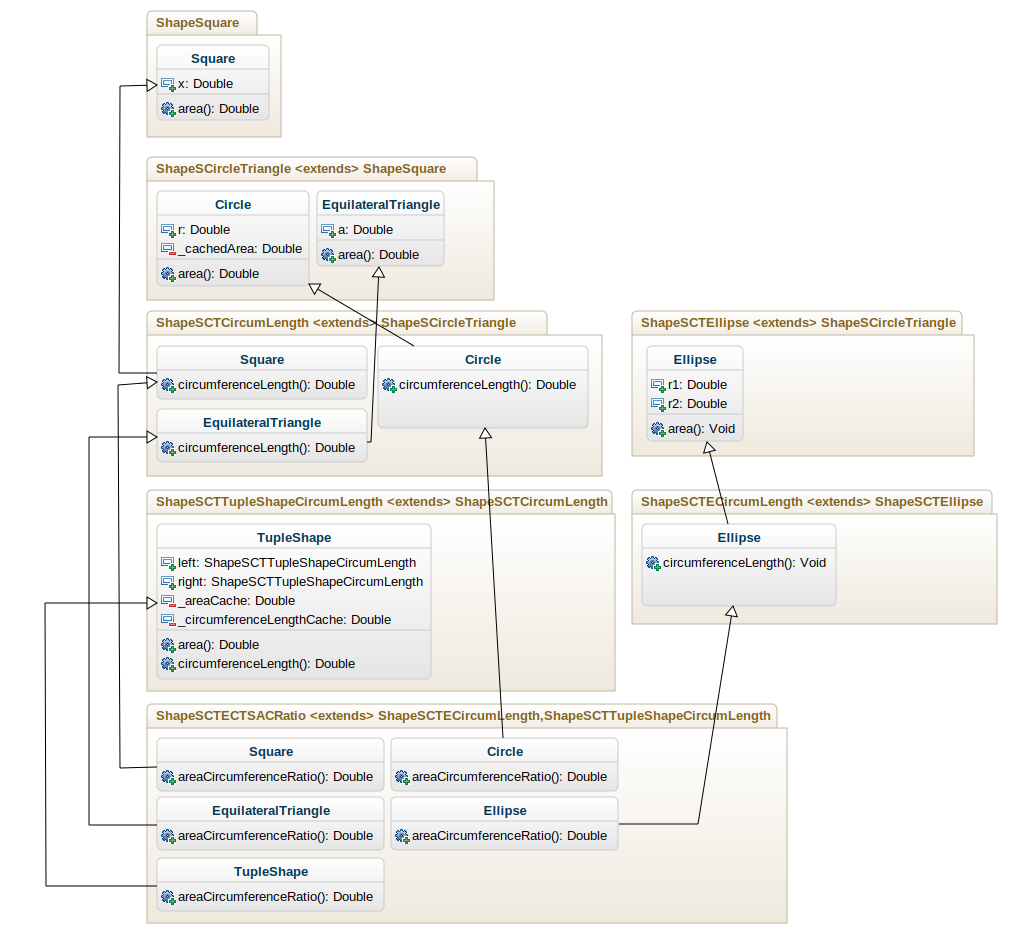
\includegraphics[width=330px,keepaspectratio=true]{Expression_problem-diag2.jpg}
\caption{Class Diagram of Use Case}
\end{figure}


\chapter*{Acknowledgements}
We want to thank 
\begingroup
\renewcommand{\cleardoublepage}{}
\renewcommand{\clearpage}{}

\bibliographystyle{plain}

\bibliography{testFile} % no suffix

\endgroup
\end{document}

















